\documentclass[tikz, border=10pt]{standalone}
\usetikzlibrary{positioning}
\usepackage{tkz-graph}
\begin{document}
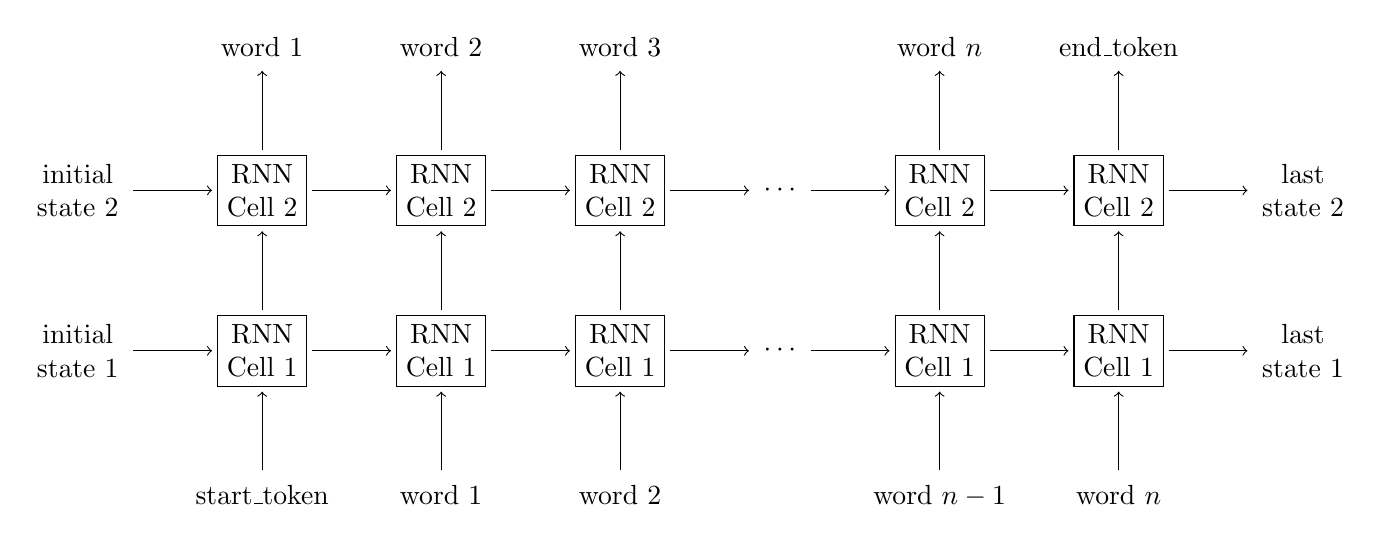
\begin{tikzpicture}

\node[align=center, outer sep=2] (x_t1) {start\_token};
\node[draw, align=center, outer sep=2] (unit_t11) [above=of x_t1] {RNN \\ Cell $1$};
\node[draw, align=center, outer sep=2] (unit_t12) [right=of unit_t11] {RNN \\ Cell $1$};
\node[draw, align=center, outer sep=2] (unit_t13) [right=of unit_t12] {RNN \\ Cell $1$};
\node[align=center, outer sep=2] (unit_t14) [right=of unit_t13] {$\cdots$};
\node[draw, align=center, outer sep=2] (unit_t15) [right=of unit_t14] {RNN \\ Cell $1$};
\node[draw, align=center, outer sep=2] (unit_t16) [right=of unit_t15] {RNN \\ Cell $1$};
\node[align=center, outer sep=2] (x_t2) [below=of unit_t12] {word $1$};
\node[align=center, outer sep=2] (x_t3) [below=of unit_t13] {word $2$};
%\node[align=center, outer sep=2] (x_t4) [below=of unit_t14] {word $3$};
\node[align=center, outer sep=2] (x_t5) [below=of unit_t15] {word $n-1$};
\node[align=center, outer sep=2] (x_t6) [below=of unit_t16] {word $n$};
\node[draw, align=center, outer sep=2] (unit_t21) [above=of unit_t11] {RNN \\ Cell $2$};
\node[draw, align=center, outer sep=2] (unit_t22) [above=of unit_t12] {RNN \\ Cell $2$};
\node[draw, align=center, outer sep=2] (unit_t23) [above=of unit_t13] {RNN \\ Cell $2$};
\node[align=center, outer sep=2] (unit_t24) [right=of unit_t23] {$\cdots$};
\node[draw, align=center, outer sep=2] (unit_t25) [above=of unit_t15] {RNN \\ Cell $2$};
\node[draw, align=center, outer sep=2] (unit_t26) [above=of unit_t16] {RNN \\ Cell $2$};
\node[align=center, outer sep=2] (unit_tprev1) [left=of unit_t11] {initial \\ state $1$};
\node[align=center, outer sep=2] (unit_tnext1) [right=of unit_t16] {last \\ state $1$};
\node[align=center, outer sep=2] (unit_tprev2) [left=of unit_t21] {initial \\ state $2$};
\node[align=center, outer sep=2] (unit_tnext2) [right=of unit_t26] {last \\ state $2$};
\node[outer sep=2] (y_t1) [above=of unit_t21] {word $1$};
\node[outer sep=2] (y_t2) [above=of unit_t22] {word $2$};
\node[outer sep=2] (y_t3) [above=of unit_t23] {word $3$};
%\node[outer sep=2] (y_t4) [above=of unit_t24] {word $4$};
\node[outer sep=2] (y_t5) [above=of unit_t25] {word $n$};
\node[outer sep=2] (y_t6) [above=of unit_t26] {end\_token};

\path[->] (x_t1) edge (unit_t11);
\path[->] (x_t2) edge (unit_t12);
\path[->] (x_t3) edge (unit_t13);
%\path[->] (x_t4) edge (unit_t14);
\path[->] (x_t5) edge (unit_t15);
\path[->] (x_t6) edge (unit_t16);
\path[->] (unit_t11) edge (unit_t21);
\path[->] (unit_t11) edge (unit_t12);
\path[->] (unit_t12) edge (unit_t22);
\path[->] (unit_t12) edge (unit_t13);
\path[->] (unit_t13) edge (unit_t23);
\path[->] (unit_t13) edge (unit_t14);
%\path[->] (unit_t14) edge (unit_t24);
\path[->] (unit_t14) edge (unit_t15);
\path[->] (unit_t15) edge (unit_t25);
\path[->] (unit_t15) edge (unit_t16);
\path[->] (unit_t16) edge (unit_t26);
\path[->] (unit_t21) edge (y_t1);
\path[->] (unit_t21) edge (unit_t22);
\path[->] (unit_t22) edge (y_t2);
\path[->] (unit_t22) edge (unit_t23);
\path[->] (unit_t23) edge (y_t3);
\path[->] (unit_t23) edge (unit_t24);
%\path[->] (unit_t24) edge (y_t4);
\path[->] (unit_t24) edge (unit_t25);
\path[->] (unit_t25) edge (y_t5);
\path[->] (unit_t25) edge (unit_t26);
\path[->] (unit_t26) edge (y_t6);
\path[->] (unit_tprev1) edge (unit_t11);
\path[->] (unit_t16) edge (unit_tnext1);
\path[->] (unit_tprev2) edge (unit_t21);
\path[->] (unit_t26) edge (unit_tnext2);

\end{tikzpicture}
\end{document}